\documentclass{article}
\usepackage[a4paper, margin=2cm]{geometry}
\usepackage{xcolor}
\usepackage{xspace}
\usepackage{booktabs}
\usepackage{dsfont}
\usepackage{footmisc}
\usepackage{marvosym}
\usepackage{amsmath}
\usepackage{hyperref}
\usepackage[capitalise,noabbrev]{cleveref}
\usepackage{tabularx}
\usepackage{listings}
\usepackage{multirow}
\usepackage{pgfplots}
\usetikzlibrary{pgfplots.statistics}
\pgfplotsset{compat=newest}

\usepgfplotslibrary{groupplots}
\pgfplotsset{every axis/.style={scale only axis}}

\pgfplotsset{
  major grid style={thin,dotted},
  minor grid style={thin,dotted},
  ymajorgrids,
  yminorgrids,
  every axis/.append style={
    line width=0.7pt,
    tick style={
      line cap=round,
      thin,
      major tick length=4pt,
      minor tick length=2pt,
    },
  },
  legend cell align=left,
  legend style={
    line width=0.7pt,
    /tikz/every even column/.append style={column sep=3mm,black},
    /tikz/every odd column/.append style={black},
  },
  % move title closer
  legend style={font=\small},
  title style={yshift=-2pt},
  % less space on left and right
  enlarge x limits=0.04,
  every tick label/.append style={font=\footnotesize},
  every axis label/.append style={font=\small},
  every axis y label/.append style={yshift=-1ex},
  /pgf/number format/1000 sep={},
  axis lines*=left,
  xlabel near ticks,
  ylabel near ticks,
  axis lines*=left,
  label style={font=\footnotesize},
  tick label style={font=\footnotesize},
  plotLeafMethods/.style={
    width=45.0mm,
    height=45.0mm,
  },
}

\title{GpuRecSplit plot}
\date{}
\begin{document}

% IMPORT-DATA leafMethods brute-force-vs-rotations.txt

% Make Pareto
%% SQL DELETE FROM leafMethods AS scatterplot
%%    WHERE EXISTS (SELECT * FROM leafMethods d
%%           WHERE d.leafMethod == scatterplot.leafMethod
%%                    AND d.bitsPerElement < scatterplot.bitsPerElement
%%                    AND d.constructionTimeMilliseconds < scatterplot.constructionTimeMilliseconds)

% Search for data points right and left of point to calculate speedups
% SQL ALTER TABLE leafMethods ADD nextLargerBruteforceSpace REAL
% SQL ALTER TABLE leafMethods ADD nextLargerBruteforceDuration REAL
% SQL ALTER TABLE leafMethods ADD nextSmallerBruteforceSpace REAL
% SQL ALTER TABLE leafMethods ADD nextSmallerBruteforceDuration REAL

%% SQL UPDATE leafMethods SET
%%   nextLargerBruteforceSpace = (SELECT bitsPerElement FROM leafMethods o WHERE o.leafMethod=="bruteforce" AND o.bitsPerElement >= leafMethods.bitsPerElement ORDER BY o.bitsPerElement ASC LIMIT 1),
%%   nextLargerBruteforceDuration = (SELECT constructionTimeMilliseconds FROM leafMethods o WHERE o.leafMethod=="bruteforce" AND o.bitsPerElement >= leafMethods.bitsPerElement ORDER BY o.bitsPerElement ASC LIMIT 1),
%%   nextSmallerBruteforceSpace = (SELECT bitsPerElement FROM leafMethods o WHERE o.leafMethod=="bruteforce" AND o.bitsPerElement <= leafMethods.bitsPerElement ORDER BY o.bitsPerElement DESC LIMIT 1),
%%   nextSmallerBruteforceDuration = (SELECT constructionTimeMilliseconds FROM leafMethods o WHERE o.leafMethod=="bruteforce" AND o.bitsPerElement <= leafMethods.bitsPerElement ORDER BY o.bitsPerElement DESC LIMIT 1)

% We calculate speedups as interpolation between the previous and next point
% SQL ALTER TABLE leafMethods ADD interpolationFactor REAL
% SQL UPDATE leafMethods SET interpolationFactor = (bitsPerElement - nextSmallerBruteforceSpace) / (nextLargerBruteforceSpace - nextSmallerBruteforceSpace)
% SQL UPDATE leafMethods SET interpolationFactor = 0 WHERE interpolationFactor IS NULL

    \centering
    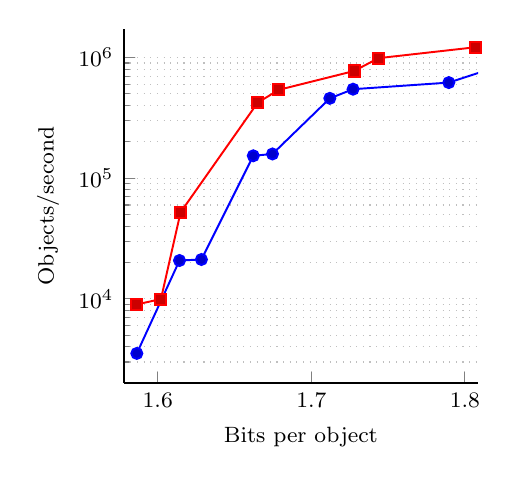
\begin{tikzpicture}
        \begin{axis}[
            xlabel={Bits per object},
            ylabel={Objects/second},
            plotLeafMethods,
            xmax=1.8,
            ymode=log,
            legend to name=paretoLeafMethodsLegend,
            legend columns=1,
          ]
          %% MULTIPLOT(leafMethod|ptitle)
          %% SELECT
          %%    bitsPerElement as x,
          %%    1000.0*N/constructionTimeMilliseconds as y,
          %%    IIF(leafMethod=="bruteforce","Brute force", IIF(leafMethod=="cuckoo", "ShockHash", IIF(leafMethod=="rotations", "Rotation fitting", leafMethod))) AS ptitle,
          %%    MULTIPLOT
          %% FROM leafMethods where leafMethod NOT LIKE "cuckoo%"
          %% ORDER BY MULTIPLOT,x
          \addplot coordinates { (1.58637,3533.58) (1.61416,20800) (1.62844,21203.1) (1.6622,153304) (1.67471,158755) (1.71205,458716) (1.72717,546150) (1.78952,619579) (1.86407,1.26422e+06) (1.8785,1.91939e+06) (1.94557,2.53165e+06) (2.14673,2.7248e+06) (2.21035,4.56621e+06) };
          \addlegendentry{Brute force};
          \addplot coordinates { (1.58639,9004.55) (1.60207,9963.04) (1.61487,52167.6) (1.66508,422654) (1.67887,539957) (1.72783,772798) (1.74369,987167) (1.80706,1.21655e+06) (1.93191,1.52439e+06) (1.94266,2.457e+06) (2.01688,3.77358e+06) (2.31285,4.7619e+06) };
          \addlegendentry{Rotation fitting};
        \end{axis}
    \end{tikzpicture}
    \hfill
    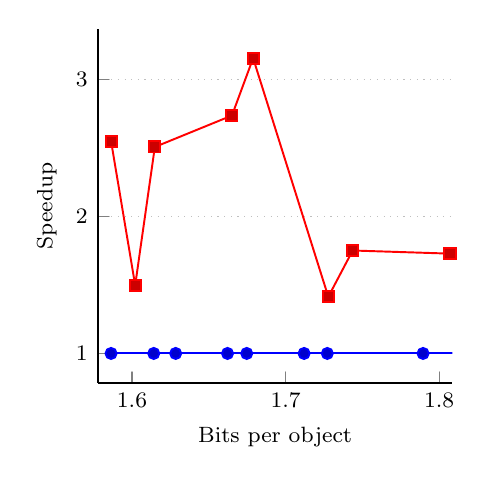
\begin{tikzpicture}
        \begin{axis}[
            xlabel={Bits per object},
            ylabel={Speedup},
            plotLeafMethods,
            xmax=1.8,
          ]
          %% MULTIPLOT(leafMethod|ptitle)
          %% SELECT
          %%    bitsPerElement as x,
          %%    1.0*(nextSmallerBruteforceDuration + interpolationFactor * (nextLargerBruteforceDuration - nextSmallerBruteforceDuration))/constructionTimeMilliseconds as y,
          %%    leafMethod AS ptitle,
          %%    MULTIPLOT
          %% FROM leafMethods scatterplot where leafMethod NOT LIKE "cuckoo%"
          %% ORDER BY MULTIPLOT,x
          \addplot coordinates { (1.58637,1.0) (1.61416,1.0) (1.62844,1.0) (1.6622,1.0) (1.67471,1.0) (1.71205,1.0) (1.72717,1.0) (1.78952,1.0) (1.86407,1.0) (1.8785,1.0) (1.94557,1.0) (2.14673,1.0) (2.21035,1.0) };
          \addlegendentry{bruteforce};
          \addplot coordinates { (1.58639,2.54676) (1.60207,1.49724) (1.61487,2.50569) (1.66508,2.73518) (1.67887,3.15341) (1.72783,1.41322) (1.74369,1.75074) (1.80706,1.72794) (1.93191,0.641253) (1.94266,0.983948) (2.01688,1.45311) };
          \addlegendentry{rotations};

          \legend{};
        \end{axis}
    \end{tikzpicture}
    \hfill
    \begin{tikzpicture}[baseline=-2cm]
        \ref*{paretoLeafMethodsLegend}
    \end{tikzpicture}

\end{document}

